% %%%%%%%%%%%%%%%%%%%%%%%%%%%%%%%%%%%%%%%%%%%%%%%%%%%%%%%%%%%%%%%%%%%%%%%%%%%%%
% thesis.tex: Primary TeX control file for thesis.
% %%%%%%%%%%%%%%%%%%%%%%%%%%%%%%%%%%%%%%%%%%%%%%%%%%%%%%%%%%%%%%%%%%%%%%%%%%%%%
\documentclass[11pt, oneside]{mnthesis}
\usepackage{epsfig} % Allows the inclusion of eps files
\usepackage{epic} % Enhanced picture mode
\usepackage{eepic} % Extensions for epic
\usepackage{units} % SI unit typesetting
\usepackage{url} % URL handling
\usepackage{longtable} % Tables that continue onto multiple pages
\usepackage{mathrsfs} % Support for \mathscr script
\usepackage{multirow} % Span rows in tables
\usepackage{bigstrut} % Space struts in tables up and down
\usepackage{amssymb} % AMS math symbols and helpers
\usepackage{graphicx} % Enhanced graphics support
\usepackage{setspace} % Adjust spacing in captions, single by default
\usepackage{xspace} % Automatically adjusting space after macros
\usepackage{amsmath} % \text, and other math formatting options
\usepackage{siunitx} % \num{} formatting and SI unit formatting
\usepackage{booktabs} % Enhanced tables with \toprule, etc.
\usepackage{hyperref} % Add clickable links to other parts of the document
\usepackage[noabbrev,capitalize]{cleveref} % Automatically determine \cref type

\usepackage[hang,flushmargin]{footmisc} % Prevent indent in footnotes. 

% Put captions tighter to their figures. Not clear if it actually works. 
\setlength{\abovecaptionskip}{0pt}

\usepackage{xcolor} % so we can put todo notes in color. 

\usepackage{doi} % Link to doi in the bibliography. Doesn't seem to work. 

\usepackage{parskip} % http://ctan.org/pkg/parskip vskip instead of indent. 

\usepackage{float} % Sometimes you want to tell LaTeX to put an image RIGHT HERE. 


% Configure the siunitx package
\sisetup{
    group-separator = {,}, % Use , to separate groups of digits, like 12,345
    list-final-separator = {, and } % Always use the serial comma in \SIlist
}

% Configure the cleveref package
\newcommand{\creflastconjunction}{, and } % Always use the serial comma




\newcommand{\Alfven}{Alfv\'en\xspace}

\newcommand{\Ampere}{Amp\`ere\xspace}

\newcommand{\xhat}{\ensuremath{\hat{x}}\xspace}
\newcommand{\yhat}{\ensuremath{\hat{y}}\xspace}
\newcommand{\zhat}{\ensuremath{\hat{z}}\xspace}

\DeclareSIUnit\RE{R_E}

\renewcommand{\vec}[1]{\underline{#1}}

\newcommand{\tensor}[1]{\underline{\underline{#1}}}

\newcommand{\dd}[1]{\ensuremath{ \frac{\partial}{\partial #1} }\xspace}

\newcommand{\ddt}{\dd{t}\xspace}

\newcommand{\dt}{\ensuremath{\delta \hspace{-0.1em} t} \xspace}

\newcommand{\curl}[1]{\ensuremath{ \nabla \times \vec{#1} }\xspace}

\newcommand{\lr}[1]{ \left( #1 \right) }

\newcommand{\lrsmall}[1]{ \left( {\scriptstyle #1} \right) }

\renewcommand{\arg}[1]{\!\lr{#1}}

\newcommand{\argsmall}[1]{\!\lrsmall{#1}}



\newcommand{\mmm}[9]{ \left[ \begin{array}{ccc}
    #1 & #2 & #3 \\
    #4 & #5 & #6 \\
    #7 & #8 & #9
  \end{array} \right] }

\newcommand{\mm}[4]{ \left[ \begin{array}{cc}
    #1 & #2 \\
    #3 & #4
  \end{array} \right] }

\newcommand{\vv}[2]{ \left[ \begin{array}{c}
    #1 \\
    #2
  \end{array} \right] }






% Note: Do we want to squish dt together? Do we want to always have tiny spaces
% between variables being multiplied together? 
\newcommand{\deltat}{\delta \hspace{-0.1em} t}


% Physics constants
\newcommand{\C}{{\mathrm{c}}}

% Add space between rows of tables
\newcommand{\spacerows}[1]{\renewcommand{\arraystretch}{#1}}

% Define a better looking eV by moving the V slightly left
\DeclareSIUnit\electronvolt{e\hspace{-0.08em}V}


\linespread{1.3}

% Compile only the chapters listed here. This may make the compile faster, but
% it's not necessary. 
%\includeonly{
%    preliminaries/title,
%    chapters/intro,
%    chapters/model,
%    chapters/math,
%    chapters/results,
%    chapters/data,
%    chapters/conclusion,
%    chapters/app_geometry,
%    chapters/app_integrating,
%}



% %%%%%%%%%%%%%%%%%%%%%%%%%%%%%%%%%%%%%%%%%%%%%%%%%%%%%%%%%%%%%%%%%%%%%%%%%%%%%
% %%%%%%%%%%%%%%%%%%%%%%%%%%%%%%%%%%%%%%%%%%%%%%%%%%%%%%% Mark this as a draft. 
% %%%%%%%%%%%%%%%%%%%%%%%%%%%%%%%%%%%%%%%%%%%%%%%%%%%%%%%%%%%%%%%%%%%%%%%%%%%%%
\draft
% %%%%%%%%%%%%%%%%%%%%%%%%%%%%%%%%%%%%%%%%%%%%%%%%%%%%%%%%%%%%%%%%%%%%%%%%%%%%%
% %%%%%%%%%%%%%%%%%%%%%%%%%%%%%%%%%%%%%%%%%%%%%%%%%%%%%%%%%%%%%%%%%%%%%%%%%%%%%
% %%%%%%%%%%%%%%%%%%%%%%%%%%%%%%%%%%%%%%%%%%%%%%%%%%%%%%%%%%%%%%%%%%%%%%%%%%%%%



\begin{document}
%\bibliographystyle{hunsrt} % style of bibliography
\bibliographystyle{abbrv} % style of bibliography

% Title and other sections that come before the body of the document
\include{preliminaries/title}

% %%%%%%%%%%%%%%%%%%%%%%%%%%%%%%%%%%%%%%%%%%%%%%%%%%%%%%%%%%%%%%%%%%%%%%%%%%%%%
% %%%%%%%%%%%%%%%%%%%%%%%%%%%%%%%%%%%%%%%%%%%%%%%%%%%%%%%%%%%%%%%%%%%%%%%%%%%%%
% %%%%%%%%%%%%%%%%%%%%%%%%%%%%%%%%%%%%%%%%%%%%%%%%%%%%%%%%%%%%%%%%%%%%%%%%%%%%%

\chapter{Introduction}
  \label{ch_intro}

\todo{In 1859, humanity was working hard to get its shit together.} The United States moved steadily toward the American Civil War, which would abolish slavery and consolidate the power of the federal government. A slew of conflicts in Southern Europe, such as the Austro-Sardinian War, set the stage for the unification of Italy. The Taiping Civil War -- one of the bloodiest conflicts of all time -- is considered by many to mark the beginning of modern Chinese history. Origin of Species was published. The first transatlantic telegraph cable was laid.

Meanwhile, ambivalent to humanity, the Sun belched an intense burst of charged particles and magnetic energy directly at Earth. The resulting geomagnetic storm\footnote{The Solar Storm of 1859 is also called the Carrington Event, after English astronomer Richard Carrington. He drew a connection between the storm's geomagnetic activity and the sunspots he had observed the day before.} caused telegraph systems to fail across the Western hemisphere\cite{green_2006}, electrocuting some operators. Displays of the northern lights were visible as far south as Cuba. 

The Solar Storm of 1859 was perhaps the most powerful in recorded history, but by no means was it a one-time event. The Sun discharges hundreds of coronal mass ejections (CMEs) per year, of all sizes, in all directions. In fact, a comparably large CME narrowly missed Earth in 2012\cite{nasa_2012}. Had it not, it's estimated\cite{lloyds_2013} that it would have caused widespread, long-term electrical outages, with a damage toll on the order of \num{e9} dollars. 

The Sun's extreme -- and temperamental -- effect on Earth's magnetic environment makes a compelling case for the ongoing study of space weather. Such research has evolved over the past century from sunspot counts and compass readings to multi-satellite missions and supercomputer simulations. Modern methods have dramatically increased humanity's understanding of the relationship between the Sun and the Earth; however, significant uncertainty continues to surround geomagnetic storms, substorms, and the various energy transport mechanisms that make them up. 

The present work focuses in particular on the phenomenon of field line resonance: \Alfven waves bouncing between the northern and southern hemispheres. Such waves play an important part in the energization of magnetospheric particles, the transport of energy from high to low altitude, and the driving of currents at the top of the atmosphere. 

%\todo{The storm of 1859 presented compelling evidence that the Sun drives geomagnetic activity. In the decades that followed, a model took shape to describe the mechanisms of energy transfer between the Sun and the Earth. Based on auroral observations and data from ground-based magnetometers, Birkeland argued for the existence of a constant outflow of electrons and ions from the Sun -- the solar wind. The advent of high-frequency radio communication allowed Kennelly, Heaviside, and others to probe the electrical properties of the upper atmosphere. }

%\todo{The study of space weather was revolutionized by the development of sounding rockets and satellites in the mid twentieth century. This allowed direct observation of the structure of the near-Earth environment, including, crucially, the waves that carry energy through it. }

%\todo{Not least among these advances was the discovery of \Alfven waves. {\Alfven}ic aurora. Carry energy and particles. }

%The study of space weather revolves around the transfer of energy from the Sun to the Earth. Ultra low frequency waves in particular are an important energy transport mechanism between the magnetosphere's outer boundary (at the solar wind) and its inner boundary (at the top of the atmosphere). 



  




\section{The Near-Earth Environment}

\todo{Sketch out the goneral structure of the magnetosphere, from the ionospheric current sheet (is this too generous?) to the magnetopause (a real current sheet). Talk about where gravity dominates, where field line curvature becomes apparent, and where the moon sits in all this. }

One hundred kilometers above Earth's surface, more or less, the neutral atmosphere transitions sharply into the conducting ionosphere.

From \cite{paschmann_2003}: ``In the thermosphere, the solar ultraviolet (UV) light and energetic particles precipitating from the magnetosphere produce ionization increasing with altitude. At the same time the particle density is low enough to make the recombination times of the ionized atoms and molecules sufficiently long to allow a significant fraction of the gas to remain ionized. This produces a conducting layer of the atmosphere known as the ionosphere. The ionosphere begins at $\sim\SI{65}{\km}$, has a peak plasma density between 200 and 300 km, and eventually merges with magnetospheric regions $\sim$1000--2000 km altitudes.''

The ionospheric E region is collisionally coupled to the neutrals. This decouples the ion and electron drifts, allowing currents to flow perpendicular to the magnetic field. 

\todo{\Alfven waves couple the magnetosphere to the ionosphere\cite{paschmann_2003}. Waves travel down the field line, accelerating particles to match the magnetospheric driver (for example, increased flow velocity as a result of enhanced reconnection). Bounces off of the ionosphere. May also bounce off the driver. Builds up drag and brings about equilibrium. }

\todo{Definition of a substorm comes from \cite{akasofu_1964}. \cite{mcpherron_1973_substorms} added the growth phase (previously it was just expansion and recovery). }

300

1000

3000

10,000 (2RE geocentric)

30,000 (5 RE)

Moon is at 60 RE or so. 

Tail goes back to about 100 RE. 

Ionosphere is dense enough to be shaped by gravity, but as altitude increases, magnetic field dominates.

The nitrogen density (w at sea level) drops from x at 100km to y at 1000km to z at 10**4 km.

By 10**4 km, the curvature of Earth's dipole magnetic field becomes apparent... and, between the increasing ion abundance and the decreasing strength of gravity, it dominates particle behavior.

At 10**5 km, the bow shock. On the dayside, at least. Balance between Earth's magnetic field and that of the sun. Another current sheet... This one far more intense.

Still less than halfway to the moon. That's 3e5 km.

This all takes place well within the orbit of the moon. Moon is about 60 RE away

Where are satellites? Geosynthronous? 

This with is concerned with the behavior of electromagnetic waves that propagate inside the magnetosheath, but outside the ionosphere; in fact, they play a significant role in the transport of energy from the former to the latter. 

Free electron density...

Still mostly neutrals, but collisions are so rare that they don't matter. At x, the mean free path of a neutral atom is comparable to... 

%There are a lot of interrelated things going on, so it's hard to describe Earth's environment one step at a time. Look at Scott's thesis -- he did this well, right? 

%Heliosphere, Magnetosphere, Ionosphere, Atmosphere?

%Typical solar wind density is $\sim$ \SI{5}{/\cm\cubed}. Typical solar wind velocity at Earth is \SIrange{e2}{e3}{\km/\s}. Typical solar wind particle energy is \SIrange{1}{10}{\kilo\eV}. Density can vary by $\sim$3 orders of magnitude, and velocity by one, during times of high solar activity. CMEs can also mess with the north/south component of the interplanetary magnetic field. 

At Earth's orbit, the solar magnetic field makes more-or-less a \SI{45}{\degree} angle with the \X axis. 
\footnote{Uppercase \X, \Y, and \Z are used to indicate GSE coordinates: \X points from the Earth to the Sun; \Y is perpendicular to \X in the Sun's ecliptic plane, pointing duskwards; \Z points north, out of the ecliptic plane. In later chapters, lowercase \x, \y, and \z are used to define a more-or-less analogous corodinate system with respect to Earth. }

% Solar wind is what deforms Earth's magnetic field to form the magnetosphere. 

% Transient solar wind phenomena, such as coronal mass ejections, are also known to be related to geomagnetic disturbances at Earth. Jesse cites here: 

% R. L. McPherron. Physical processes producing magnetospheric substorms and mangetic storms. In J. A. Jacobs, editor, Geomagnetism, volume 4, chapter 7. Academic Press, 1991.

% G. Rostoker. Substorms. In Handbook of the Solar-Terrestrial Environment, chapter 15. Springer-Verlag, 2007.

% This might just be worth tracking down... Jesse cites several chapters: 

% M. Shulz. Magnetospheres. In Handbook of the Solar-Terrestrial Environment, chapter 7. Springer-Verlag, 2007.

% papers mentioned during Yan's talk. mostly about alfven acceleration and nonlinear effects. 
% Vasyliunas 1970, 1984
% Hasegawa 1976
% Goertz 1991
% Stasiewicz et al 2000
% Haerendel 2008
% Song & Lysak 1994, 1999, 2000, 2001, 2006, 2011, 2012
% Inverted V?
% Double layers? 
% Charge holes? 

% -----------------------------------------------------------------------------
% -----------------------------------------------------------------------------
% -----------------------------------------------------------------------------
\subsection{The Outer Magnetosphere}


Significant deformation by the solar wind. 

Bow shock. 

Magnetopause. Current sheet consistent with \amplaw. 

Plasma sheet and PSBL. 

Tail and tail lobes. 

Reconnection. 


% -----------------------------------------------------------------------------
% -----------------------------------------------------------------------------
% -----------------------------------------------------------------------------
\subsection{The Inner Magnetosphere}

Closed field lines. More or less dipolar. 

The plasmasphere and plasmapause. 

Radiation belts. Radial diffusion is interesting because... 

\Alfven speed. So we probably want to at least mention field line resonance here? Or do we get into that in the next chapter? Plot of \Alfven speeds and \Alfven bounce times for each profile. 


% -----------------------------------------------------------------------------
% -----------------------------------------------------------------------------
% -----------------------------------------------------------------------------
\subsection{The Ionosphere}
  \label{sec_ionos}

Pedersen, Hall, and field-aligned conductivity. Do we want to get into two-cell convection? Region 1 and 2 current? 

\todo{Convection electric field. How close to Earth does it get? Don't we lose $\vec{E}=\cross{V}{B}$ when there are currents? }

``Increasing the Hall conductance allows the energy to oscillate through the inductive process rather than dissipate as Joule heating, increasing the `ringtime' of field line resonances.''\cite{waters_2013}

Scale heights. Ion/neutral composition. 

E, F layers. 

Ionospheric \Alfven resonator. This is important if we want to talk briefly about all kinds of ULF waves. 

Precipitation. Inverted V. 

\todo{Scott's thesis has a TON of detail. How much does Jesse show? }

\begin{figure}[H]
    \centering
    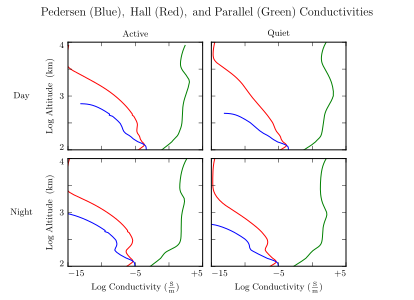
\includegraphics[width=\textwidth]{figures/sigma.pdf}
    \caption[Ionospheric Conductivity Profiles]{
      Ionospheric conductivity profiles, adapted by Lysak\cite{lysak_2013} from Appendix B of Kelley's textbook\cite{kelley_1989}. 
    }
    \label{fig_sigma}
\end{figure}


\begin{longtable}{ @{\extracolsep{\fill}} lrrr @{\extracolsep{\fill}} }
  \caption[Integrated Atmospheric Conductivity]{Integrated Atmospheric Conductivity (\si{\S})}
  \label{tab_sigma_atm} \\

  \toprule
  &
  $\Sigma_0$ &
  $\Sigma_P$ &
  $\Sigma_H$ \\
  \midrule
  \endfirsthead

  % Footer for the end of the table
  \bottomrule
  \endlastfoot

  Active Day &
  424 &
  0.65 &
  6.03 \\

  Quiet Day &
  284 &
  0.44 &
  4.02 \\

  Active Night &
  9 &
  0.01 &
  0.12 \\

  Quiet Night &
  9 &
  0.01 &
  0.12 \\

\end{longtable}

\begin{longtable}{ @{\extracolsep{\fill}} lrrr @{\extracolsep{\fill}} }
  \caption[Integrated Ionospheric Conductivity]{Integrated Ionospheric Conductivity (\si{\S})}
  \label{tab_sigma_ionos} \\

  \toprule
  &
  $\Sigma_0$ &
  $\Sigma_P$ &
  $\Sigma_H$ \\
  \midrule
  \endfirsthead

  % Footer for the end of the table
  \bottomrule
  \endlastfoot

  Active Day &
  --- &
  13.0 &
  17.0 \\

  Quiet Day &
  --- &
  5.6 &
  10.2 \\

  Active Night &
  --- &
  0.8 &
  0.3 \\

  Quiet Night &
  --- &
  0.2 &
  0.3 \\

\end{longtable}


\todo{Get this working... }



  % =============================================================================
% =============================================================================
% =============================================================================
\section{Geomagnetic Disturbances}
  \label{sec_storms}

% -----------------------------------------------------------------------------
% -----------------------------------------------------------------------------
% -----------------------------------------------------------------------------
\subsection{Storms}

% -----------------------------------------------------------------------------
% -----------------------------------------------------------------------------
% -----------------------------------------------------------------------------
\subsection{Substorms}

Storms! CMEs, etc. 

\todo{Definition of a substorm comes from \cite{akasofu_1964}. \cite{mcpherron_1973_substorms} added the growth phase (previously it was just expansion and recovery). }

What causes a storm. 

Storm effects: outer magnetosphere, inner magnetosphere, on the ground.

The ionospheric profiles used in this model are based on values tabulated in the Appendix B of Kelley's book\cite{kelley_1989}. They were adapted by Lysak\cite{lysak_2013} to take into account the effect of the magnetosphere's latitude-dependent density profile. 

Mean molecular mass of \SI{28}{\amu} at \SI{100}{\km}, \SI{16}{\amu} around \SI{400}{\km}, down to \SI{1}{\amu} above \SI{1400}{\km}. 

Simulations are carried out using four profiles: active day, quiet day, active night, quiet night. 

Profiles are static for the duration of a simulation. Even so-called ultra low frequency waves are still much faster than convective timescales. 

\todo{Come up with a characteristic convective timescale or two, and cite it. }

The effects of mean molecular mass on conductivity are computed per the usual definitions. 
\begin{align}
  \sp &= \displaystyle\sum_s \frac{n_s q_s^2}{m_s} \frac{\nu_s}{\nu_s^2 + \Omega_s^2} &
  \sh &= -\displaystyle\sum_s \frac{n_s q_s^2}{m_s} \frac{\Omega_s}{\nu_s^2 + \Omega_s^2} &
  \sz &= \displaystyle\sum_s \frac{n_s q_s^2}{m_s \nu_s}
\end{align}

Each profile is resolved to an altitude of about $\SI{e4}{\km}$, and include well-resolved $E$, $F_1$, and $F_2$ layers. 










  % =============================================================================
% =============================================================================
% =============================================================================
\section{Field Line Resonance}
  \label{sec_flrs}


%
% From W J Hughes' Magnetospheric ULF Waves: A Tutorial With a Historical Perspective
%

% rolf 1920 for early observation of Pi2

% Patel 1965 made observations in space, and matched them to observations on the ground
% Cummings et al 1969 numerically integrated Dungey's equations to estimate eigenfrequencies
% soviets discovered that different pulsations have different sources in the 1970s; see troitskaya 1993 and greenstadt and russell 1993
% troitskaya 1969 showed that Pc3 can sometimes be explained by a sudden change in the size of the magnetosphere following an impulse. an example -- this must have also been seen earlier. because... 
% Bolshakova and Troitskaya 1968 showed that Pc3 observation depends on IMF N/S. Iff IMF is within about 50 degrees of the earth-sun linem Pc3 is observable on the ground. 
% Troitskaya et al 1971 showed Pc3 frequencies at L=3 depend on IMF magnitude
% Gul'elmi 1974 and Kovner et al gave theoretical justification for these observations. 
% Russell and Hoppe 1981 made observations upstream of the bow shock to unify some ideas. upstream waves are driven by ion cyclotron instability, which depends on IMF magnitude. 

% Gringauz et al 1970 found that solar wind number density affects Pc3 and Pc4 periods (oppositely). The Pc4 effect is a standing question. 

% Samson et al 1971 new observations with digital recording and arrays near the plasmapause! they showed MLT dependence of peak amplitude, and different regions of opposite circular polarization. 
% Dungey 1954 had suggested KH as a wave energy source, which explained the flipping circular polarization at noon. 
% Southwood 1974 went back to the equations and came up with a reason for resonance. waves hitting the bow shock propagate in as an evanescent fast mode. when it gets to a resonant field line, the fast mode couples to the shear mode. the energy tunnels. this only happens if dissipation is finite. 
% Chen and Hasegawa 1974 did too, independently
% Newton et al 1978 showed that joule dissipation at the ionosphere is dominant, and that the amount of dissipation determines the width of the resonance. 

% kivelson et al 1984 argued for cavity mode eigenfrequencies. Pc5. 
% kivelson and southwood 1985, 1986 did analytical work to defend it. 
% Lee and Lysak 1991 did numerical work in a dipole geometry. 

% Harrold and Samson 1992 The waves probably have to be reflected by the bow shock, not by the magnetopause, to line up with the observed eigenfrequencies. 1 to 3 mHz. 

% allan et al 1985 did early observation of ULF waves (Pc5 and Pc4) from waveform plots. 
% Waters et al 1991 ground-based observation of Pc3 and Pc4 before spacecraft existed at small L. 
% Menk et al 1993 also




\todo{Haven't read this paper yet, but it looks fun: \cite{glassmeier_2004}. }

\todo{Fishbone instability? }

\todo{Lab \Alfven waves as LASP? }

The motion of a charged particle in a dipole field can be described in terms of three fundamental motions. First is cyclotron motion: a particle orbits around a magnetic field line. Second is bounce motion: while orbiting, the particle moves along the field line like a bead on a string, back and forth between the northern and southern hemispheres\footnote{As a particle approaches Earth, it experiences an ever-stronger magnetic field. The particle's perpendicular kinetic energy increases in proportion with the magnetic field in order to conserve its first adiabatic invariant. When the perpendicular kinetic energy can no longer increase -- that is, when the parallel kinetic energy is zero -- the particle bounces back. (If the parallel kinetic energy is sufficiently large, the particle doesn't bounce; it precipitates into the atmosphere.)}. Third is drift motion: as particles orbit and bounce, they also experience a net azimuthal motion\footnote{Particle drift is a consequence of the gradient-curvature drift in Earth's curved, nonuniform magnetic field.}. 

\todo{Electron cyclotron frequency is on the order of $\sim \SI{1}{\MHz}$ in the ionosphere, and more like $\sim \SI{1}{\kHz}$ in the magnetosphere. Much faster than drift or bounce timescales. Ion cyclotron frequency... down by a factor of $\frac{\me}{\mp}$. }

\todo{Bounce timescales are faster closer to Earth (where the field lines are short) and slower further out. Something like \SIrange{10}{100}{\second}. Bounce timescales depend only on velocity, right? }

\todo{Drift timescales vary significantly based on particle energy. Dai\cite{dai_2013} showed a nice example of \SI{100}{\kilo\eV} ions drifting with a period of $\sim \SI{100}{\s}$. Bounce and drift timescales can overlap -- this turns out to be important. This doesn't depend on mass, right? Just kinetic energy. }

\todo{Electromagnetic waves are oscillating all over the place in the magnetosphere. When wave oscillation frequency lines up with a particle's cyclotron, bounce, and/or drift period, there can be an ongoing energy exchange between the wave and the particle. Wave-particle interaction. Analogy: a surfer moves along with a wave in the ocean, continuously gaining energy from it. Particles, by ``surfing'' on electromagnetic waves, can become energized as well as radially displaced. This is a significant energy transport mechanism. }

\todo{Any waves with frequencies of $\SIrange{e-3}{1}{\Hz}$ are termed ULF waves -- ultra low frequency. ULF waves are furthermore categorized in terms of their morphological characteristics. Pc waves are continuous (exhibiting a fairly consistent waveform over a large number of wave periods) while Pi are irregular; the waves are further partitioned into frequency bands. See \cref{tab_iaga}. }

\todo{These are Jacobs' original ranges... but are they really reflective of the jargon still used? It's weird that these ranges bottom out so far below 1000s. }

\begin{longtable}{ @{\extracolsep{\fill}} cccccccc @{\extracolsep{\fill}} }
  \caption[IAGA Magnetic Pulsation Frequency Bands]{IAGA Magnetic Pulsation Frequency Bands\cite{jacobs_1964}}
  \label{tab_iaga} \\

  \toprule
  &
  Pc1 &
  Pc2 &
  Pc3 &
  Pc4 &
  Pc5 &
  Pi1 &
  Pi2 \\
  \midrule
  \endfirsthead

  % Footer for the end of the table
  \bottomrule
  \endlastfoot

  Period (\si{\second}) &
  0.2--5 &
  5--10 &
  10--45 &
  45--150 &
  150--600 &
  1--40 &
  40--150 \\

  Frequency (\si{\mHz})&
  200--5000 &
  100--200 &
  22--100 &
  7--22 &
  2--7 &
  25--1000 &
  7--25 \\

\end{longtable}

\todo{While the IAGA characterizations are based on wave morphology, they do a decent job of deliniating between the different underlying physical processes as well. Pi2 pulsations (irregular waves with periods of a minute or two) tend to be excited on the nightside; they are associated with substorm onset (though the processes that give rise to Pi2s -- and their relation to substorm onset -- remains controversial). Pc1 and Pc2 pulsations tend to be EMIC (electromagnetic ion cyclotron) waves near the ion gyrofrequency, which are important for the precipitation of electrons (?). }

Pi2: ``Clearly linked to substorm disturbances and other impulsive dynamics are the irregularly shaped waves in the 7--25-mHz band referred to as Pi2. Recent work on these waves suggests that their periodicity reflects the spectrum of global mode excitations of the plasmasphere but there is a competing proposal that the dominant frequencies are imposed by the modulated flows in the magnetotail.''\cite{kivelson_2006}

\todo{The present work is specifically concerned with field line resonances near the plasmapause. These waves fall in the Pc4 range, with frequencies around \SI{10}{\mHz}\footnote{Notably, field line resonances can also fall within the Pc3 and Pc5 ranges. }. }






The study of field line resonance dates back to Dungey's seminal work in 1954\cite{dungey_1954}, which describes the possibility of an \Alfven wave bouncing back and forth along a magnetic field line.

\todo{Field line resonance is an important energy transport mechanism! }

Drift resonance happens when the bounce frequency of an \Alfven wave between the northern and southern ionospheres matches the bounce frequency of nearby particles. It allows the energization of ring current and radiation belt particles through drift and drift-bounce resonance\cite{elkington_1999,mann_2013,ozeke_2008,southwood_1976}. By multiple wave-particle interactions, poloidal ULF waves [FLRs] can lead to radial diffusion of radiation belt particles\cite{elkington_2003,ozeke_2012,tu_2012}.


\todo{Above the profile, Bob scales the value that's read in as $r^5$ or something. Is there a citation for that? }

The \Alfven speed is then computed per $\va^2 \equiv \frac{1}{\mz \ep}$. 

The \Alfven speed is computed from Kelley's low-density profile, modified to take into account the local density. The density, in turn, is the sum of a plasmaspheric profile and a high-latitude auroral profile. 
\begin{align}
  \ep &= \text{(low-density tabulated value)} + \frac{ n \bar{m} }{B_0^2}
\end{align}

Where $\bar{m}$ is the ambient mean molecular mass and $B_0$ is the zeroth-order magnetic field strength, $B_0 = \SI{3.11e4}{\nano\tesla} \lr{ \frac{R_E}{r} }^3 \sqrt{ 1 + 3 \cos^2 \theta }$. Note that \SI{3.11e4}{\nano\tesla} is the value of the Earth's magnetic field at the equator on Earth's surface. 

\todo{Does Kelley list the electric constant or the \Alfven speed? }

\begin{figure}[H]
    \centering
    \includegraphics[width=\textwidth]{figures/fa.pdf}
    \caption[\Alfven Bounce Frequency Profiles]{
      \Alfven bounce frequency profiles, computed by integrating the the \Alfven speed back and forth over a field line. $f_A = \lrb{ \oint \frac{dz}{v_A} }^{-1}$. Dotted lines indicate the Pc4 frequency range, \SIrange{7}{25}{\mHz}. In each profile, the effect of the plasmapause is clearly visible, centered at $L=4$. Field lines just inside and just outside the plasmapause appear susceptible to resonance in the Pc4 band. 
    }
    \label{fig_fa}
\end{figure}

\todo{Talk about how the size of the plasmasphere can be adjusted, and \SI{4}{\RE} is just a typical value. }

ULF waves have been shown to correlate with pulsating aurora and with chorus\cite{jaynes_2015}. It's believed that (in the case presented) substorm injection drove Pc4-5 pulsations, which modulated chorus waves, which pitch-angle scattered electrons with energies on the order of \SI{10}{\kilo\eV}. 

\todo{Early observations of field line resonance. }

Ground signatures in the Pc4 range identified in the 1930s\cite{angenheister_1931}. Decades later, simultaneous observations at conjugate foot points of the same field line showed FLR structure\cite{sigura_1961}. And looked at their structure (?) \cite{nagata_1963}. 

\todo{Modern observations -- how do we justify using a 2.5D model? Localization in MLT. }

Pc4 pulsations are radially localized, per multiple satellite observations\cite{engebretson_1992}, and spread no more than about 8 hours MLT. They peak around $L$ of 5 to 6, with lower occurrence rate 2.5 to 9\cite{anderson_1990,liu_2009}.

\todo{Radial localization. }

The plasmapause -- representing a sharp change in \Alfven speed -- is important for ULF waves. Waves are trapped and scattered by the effective potential well, analogous to \Schrodinger's equation\cite{lee_1998,lee_1999,dai_2009}. This has been shown theoretically\cite{klimushkin_1998,leonovich_2000,klimushkin_2004,mager_2013} (most recent is \cite{mager_2013}) and observationally\cite{takahashi_2009,takahashi_2010}. 

\todo{On the generation of FLRs: }

Compressional waves come from the outer boundary, propagating across field lines\cite{lysak_1992}. 

Compressional driving doesn't preclude drift or drift-bounce resonance\cite{zong_2007,zong_2009}. 

Plasmapause refilling may cause onset of the instability that drives noncompressional Pc4s\cite{engebretson_1992,liu_2013}. 

Low \azm is compressional\cite{hughes_1994}. Drivers may include KH at the magnetopause\cite{chen_1974,southwood_1974,liu_2011}, variations in solar wind pressure (such as interplanetary shocks)\cite{zong_2007,zong_2009,hao_2014,degeling_2014,kessel_2008}, and waves in the foreshock region\cite{russell_1983,takahashi_2015}. 

AMPTE/CCE data has shown a correlation between poloidal Pc4 activity and intense ring current flux near the equator\cite{engebretson_1988}. Poloidal Pc4s may be caused by phase space gradients\cite{dai_2013}. Fundamental standing waves are possibly excited by drift resonance of ions with energy around \SI{100}{\kilo\eV}\cite{thompson_2001,dai_2013}.

``To summarize, the general buffetting of the magnetosphere by variations in the solar wind dynamic pressure, or perhaps by sporadic magnetic reconnection, provides a broad band energy source to the magnetosphere. The magnetospheric cavity as a whole rings at its own eigenfrequencies, thus transporting energy at just those frequencies to field lines deep in the magnetosphere. Those field lines whose eigenfrequencies match one of the cavity eigenfrequencies couple to the cavity mode and resonate strongly, producing the classical field line resonance signature.\cite{hughes_1994}'' 

\todo{Observational constraints for ground-based work on FLRs: }

High-modenumber ULF pulsations are damped by the ionosphere, making it more difficult to observe them on the ground\cite{hughes_1976}. Small structures are also damped; resonances narrower than $\sim \SI{100}{km}$ aren't visible on the ground. See also Glassmeier and Stellmacher, 2000 (about small latitude), and Wright and Yeoman, 1999, Yeoman and Wright, 2001 about large \azm. 

Second harmonic poloidal waves -- as most of \cite{dai_2015}'s events are -- are unlikely to cause a Pg event on the ground\cite{takahashi_1992}. 

It's perhaps not surprising that, finding events based on ground signatures, \azm would skew low. High-\azm waves can't penetrate the ionosphere. Multi-spacecraft observation of a ULF wave with very high modenumber (70+) and no apparent ground signature\cite{takahashi_2013}. 

\todo{The ionosphere is important: }

A Hall-conducting ionosphere reflects ULF waves\cite{hughes_1974}. 

Poloidal and toroidal ULF polarizations are treated differently by the ionosphere\cite{greifinger_1968} (more recently, \cite{fujita_1988}).  

\todo{Theoretical consideration of decay vs propagation, by frequency. Lysak and Yoshikawa 2006. }

\Alfven waves with small latitudinal scale\cite{glassmeier_2000} or high \azm\cite{wright_1999,yeoman_2001} are screened by the ionosphere. Attenuation factor from \cite{hughes_1976} and \cite{glassmeier_1984} DID NOT PRINT PROPERLY. LOOK IT UP. 

Typical magnitude is order of a few nT, and a few mV/m\cite{takahashi_2013}. 

% -----------------------------------------------------------------------------
% -----------------------------------------------------------------------------
% -----------------------------------------------------------------------------
\subsection{Structure and Jargon}

\todo{Poloidal and toroidal, fundamental mode and second harmonic... make sure this vocabulary is inescapably clear! }

Drift-wave instability\cite{hasegawa_1971,green_1979,green_1985} is also a possibility for exciting fundamental poloidal waves, though it requires cold plasma, so it could only happen in the plasmasphere. 

Fundamental poloidal mode is drift resonance, not drift bounce\cite{poulter_1983}. 

Pc5 waves peak around $L$ of 7 to 9, too far out for RBSP\cite{anderson_1990,liu_2009}. Poloidal Pc4 pulsations are common inside and outside the plasmapause. Plasmapause peaks at 4.8--5 RE and 5.8--6RE\cite{dai_2015}. 

Because the inner magnetosphere is low-$\beta$ (that is, magnetic pressure dominates thermal pressure), the strength of the compressional-poloidal coupling indicates \azm\cite{hughes_1994}. 

At high \azm, the poloidal mode decouples from the compressional mode\cite{hughes_1994} and becomes guided\cite{cummings_1969}. 

Most observed guided waves are second harmonic excited by the drift-bounce resonance\cite{hughes_1978,singer_1982,takahashi_1990}. Fundamental modes, driven by drift resonance, are rarer, but have been observed\cite{dai_2013}. The energy of the resonant particle gives \azm, recall $\omega - \azm \omega_d = 0$ or something\cite{ozeke_2001}. 

A recent survey of Van Allen Probe data showed that Pc4 pulsations -- the poloidal ones, at least -- occur primarily during geomagnetically active times, near the plasmapause, over just a handful of hours of dayside MLT\cite{dai_2015}. This confirmed and refined older work\cite{engebretson_1987}. 

In the example shown of a fundamental mode poloidal Pc4, and in the example of a higher harmonic Pc4, a mishmash of toroidal activity is present. \cite{dai_2015}, figure 8 and 9 respectively. 

Compressional poloidal Pc4 pulsations are much more common during storms, but not particularly sensitive to storm phase. Noncompressional ones occur primarily during recovery\cite{dai_2015,rostoker_1979,engebretson_1992,anderson_1994}. Note that Dai\cite{dai_2015} was pretty generous about what counted as a storm... anything that hits \SI{-30}{\nano\tesla}. So \cite{motoba_2015} may not have counted the same way when they found no particular correlation with storm phase. 
\todo{Fishbone instability. McGuire 1983, Chen 1984. Similar phenomenon, but for lab plasmas. }

An ideal poloidal mode decays to the toroidal mode in the presence of curved magnetic field lines\cite{radoski_1974} or a gradient in the \Alfven speed\cite{mann_1995}. The time is proportional to the azimuthal wavenumber\cite{mann_1995}. An analytical follow-up agreed with the numerical work\cite{mann_1997}. 

\todo{Mann gives the poloidal-to-toroidal decay time to be $\tau = \frac{d \lambda}{d \omega_A'}$, where $\lambda = \frac{\azm}{2 \pi r}$ and $\omega_A'$ is the spatial derivative of the \Alfven bounce frequency, but this doesn't seem to line up. When $\tau$ is computed using our \Alfven bounce frequencies, the result is much less than \SI{1}{\second}. Double-checking is necessary. }

\cite{cummings_1969}: Standing \Alfven waves in the magnetosphere. Theoretical fundamental toroidal and poloidal modes can vary by up to \SI{30}{\percent} in frequency. 

Second harmonic: Br leads Ea by 90 degrees. Fundamental mode: Br lags Ea by 90 degrees. DEPENDS ON SIGN OF MLAT. \cite{dai_2015}

Low-\azm waves tend to be more muddled... driven by broadband sources rather than resonance\cite{dai_2015}. 

Drift resonance is the fundamental mode. Drift-bounce is higher harmonics\cite{dai_2015}. 

\todo{Do the unambiguous Pc4 events in \cite{takahashi_2011} and \cite{dai_2013} also have a mishmash of toroidal activity? }

Fundamental mode is rare. Of 390 noncompressional events, Dai identified 19 to be clearly fundamental mode and 197 to be clearly second harmonic\cite{dai_2015}. 

Fast and shear (toroidal and poloidal) modes are coupled by nonzero Hall conductivity\cite{kato_1956}. 

Shear mode incident on the ionosphere, pederson current closes FAC, Hall current then generates a fast mode wave which may be detected in space or on the ground\cite{tamao_1965}. 

Toroidal mode is usually associated with external driving\cite{chen_1974,southwood_1974}. 

Guided poloidal wave arises as \azm goes to infinity\cite{radoski_1967_poloidal}. 

Observations show that the poloidal mode is most excited in the second harmonic\cite{cummings_1969,hughes_1978,arthur_1981,singer_1982,takahashi_1984,engebretson_1988} even when there is a strong compressional component\cite{takahashi_1987,haerendel_1999,vaivads_2001,sibeck_2012}. 

Theoretical justifications for why the second harmonic would be preferrentially excited in the ring current environment. Basically, the drift-ballooning mode is only unstable in the case of antisymmetry\cite{southwood_1976,chen_1991,cheng_1994,chan_1994}. 

Observations of odd-mode poloidal waves... possible fundamental\cite{yang_2010,eriksson_2005}.

% -----------------------------------------------------------------------------
% -----------------------------------------------------------------------------
% -----------------------------------------------------------------------------
\subsection{Giant Pulsations}

First Pg observation\cite{birkeland_1901}. 

Pc4 pulsations in general tend to exhibit meridional polarization on the ground, but giant pulsations have east-west polarization\cite{takahashi_1992}. 

Pgs are most common during solar minimum, perhaps because of decreased mass loading of heavy ions\cite{denton_2011}. 

Observations in space indicate that Pgs are fundamental poloidal mode\cite{kokubun_1980,hillebrand_1982,kokubun_1989,takahashi_1992,glassmeier_1999}. 

Pgs are rare\cite{brekke_1987}. Most Pgs observed on the ground have \azm in the range 16 to 35\cite{takahashi_1992}. Motoba\cite{motoba_2015} found \azm valuse in the range 10 to 15 for a sample of Pgs. Previous studies\cite{rostoker_1979,glassmeier_1980,hillebrand_1982,poulter_1983} are in general agreement that Pg modenumbers fall into the range 16 to 35. 

A long-period \Alfven wave passing through the ionosphere is rotated by about 90 degrees\cite{nishida_1964_screening,hughes_1974}. That would translate a poloidal resonance in space to an east-west ground signature. 

\cite{motoba_2015} suggests that Pgs originate from the fundamental poloidal mode waves at all local times. 

It seems to be the convention to find a Pg event on the ground, then look at satellite data. That's certainly what was done in \cite{motoba_2015}. 

Per \cite{motoba_2015}, most Pg events happen around $L=7$, but some do happen near the plasmapause, as seen(?) by \cite{green_1985}. 

``The AL distribution shown in Figure 14c are consistent with the findings of \cite{rostoker_1979} that Pgs occur as the magnetosphere recovers from previous activities (substorms).''\cite{motoba_2015} Finds this to be reasonable because it's ``very likely'' that energetic ions injected into the inner magnetosphere from the magnetotail provide energy to Pgs. 

Analysis of GOES data from 2008 to 2013 shows about 100 Pg events. They are concentrated on the morningside. No particular correlation with storm phase\cite{motoba_2015}. 

Recall compressional poloidal Pc4s are mostly during storm time, and noncompressional are mostly specifically during late recovery\cite{dai_2015}. Only 19 fundamental poloidal mode examples were identified from the 390 noncompressional poloidal events. 

Another past study: \cite{takahashi_1984}. Satellite data is surveyed and classified by polarization, harmonic, wavenumber, etc, in order to determine the mechanisms for generating \Alfven waves. Old, but still pretty representative, according to Motoba\cite{motoba_2015}. 

% -----------------------------------------------------------------------------
% -----------------------------------------------------------------------------
% -----------------------------------------------------------------------------
\subsection{Motivations for the Present Work}

Dai writes, in his 2015 paper\cite{dai_2015}, ``It is not clear why noncompressional [high-\azm] Pc4 poloidal waves, which are presumably driven by instability within the magnetosphere, preferrentially occur on the dayside.'' 

Motoba\cite{motoba_2015}, similarly, notes ``It is unclear whether other generation mechanisms of fundamental standing waves ... can explain the localization of Pgs in local time.''

The present work uses a numerical model to investigate the preferrential occurrence of field line resonances in the Pc4 range -- particularly first-harmonic poloidal modes, such as giant pulsations -- in MLT. 



Giant pulsations have variously been referred to as ``intriguing''\cite{green_1985}

``rare''\cite{brekke_1987}, even to the point of being ``a small subset of fundamental poloidal waves''\cite{takahashi_2013} -- note that it's well known that fundamental poloidal mode waves are already rare in comparison to second harmonic waves. 




\todo{What's going on with the MLT localization of Pc4 pulsations? Is there something spooky going on with the driving? Maybe the ionosphere just kills FLRs on the nightside! }

\todo{What's so special about Pgs? How rare are they, really, compared to fundamental poloidal modes in general? How does that line up with the occurrence rate of nice, sinusoidal waveforms in second-harmonic Pc4s? That is, is there something special about Pgs, or do they just live in a ``sweet spot'' with respect to constraints on observation and resonance? }

\todo{The goal here is to clarify and unify several constraints on the viability and observability of FLRs. }

%``Pgs maybe a manifestation of a small subset of fundamental poloidal waves excited in the magnetopause.'' \cite{takahashi_2013}

%``It is not clear why noncompressional [high-\azm] Pc4 poloidal waves, which are presumably driven by instability within the magnetosphere, preferrentially occur on the dayside.\cite{dai_2015}''

%``It is unclear whether other generation mechanisms of fundamental standing waves such as drift wave instability\cite{green_1979} can explain the localization of Pgs in local time (LT).''\cite{motoba_2015}













% %%%%%%%%%%%%%%%%%%%%%%%%%%%%%%%%%%%%%%%%%%%%%%%%%%%%%%%%%%%%%%%%%%%%%%%%%%%%%
% %%%%%%%%%%%%%%%%%%%%%%%%%%%%%%%%%%%%%%%%%%%%%% Description of Numerical Model
% %%%%%%%%%%%%%%%%%%%%%%%%%%%%%%%%%%%%%%%%%%%%%%%%%%%%%%%%%%%%%%%%%%%%%%%%%%%%%

\chapter{Model}
  \label{ch_model}

\todo{This chapter runs through the numerical model... starting with the math that underlies it, then looking at the model itself, then a cool extra thing. }







``Increasing the Hall conductance allows the energy to oscillate through the inductive process rather than dissipate as Joule heating, increasing the `ringtime' of field line resonances.''\cite{waters_2013}



Ionospheric profiles are static for the duration of a simulation. Even so-called ultra low frequency waves are still much faster than convective timescales. Each profile is resolved to an altitude of about $\SI{e4}{\km}$, and include well-resolved $E$, $F_1$, and $F_2$ layers. 


  % =============================================================================
% =============================================================================
% =============================================================================
\section{Dispersion Relation}
  \label{sec_math}

Before delving into the implementation of the numerical model, it's instructive to consider the fundamental equations of waves in a cold, resistive plasma. 

The evolution of electric and magnetic fields is governed by \amplaw and \farlaw. Notably, the present work takes the linearized versions of Maxwell's equations; the vectors \vec{E} and \vec{B} indicate perturbations above the zeroth-order magnetic field. 
\begin{align}
  \label{math_maxwells}
  \tensor{\epsilon} \cdot \ddt \vec{E} &= \oomz \curl{B} - \vec{J} & \ddt \vec{B} &= -\curl{E}
\end{align}

Current follows \ohmlaw. For currents perpendicular to the background magnetic field, Kirchhoff's formulation is sufficient. Conductivity is much higher along the magnetic field lines\footnote{The dipole coordinate system is defined rigorously in \cref{sec_coords}; at present, it's sufficient to take \zhat parallel to the zeroth-order magnetic field, and \xhat and \yhat perpendicular to \zhat (and to each other). }, so it's appropriate to also include the electron inertial term\footnote{Electron inertial effects are not included in the model described in \cref{sec_tuna}, or in the results in \cref{ch_results}; however, their implementation and impact are explored in \cref{sec_inertia}. }. 
\begin{align}
  \label{math_ohms}
  0 &= \tensor{\sigma}_\bot \cdot \vec{E}_\bot - \vec{J}_\bot &
  \frac{\me}{n e^2} \ddt J_z &= \sz E_z - J_z
\end{align}

The derivatives in \cref{math_maxwells,math_ohms} can be evaluated by performing a Fourier transform. They can then be combined, eliminating the magnetic field and current terms. 
\begin{align}
  \label{disp_setup}
\begin{alignedat}{4}
  & 0 = \vec{E}_\bot && + \frac{\va^2}{\omega^2} \lr{ \vec{k} \times \vec{k} \times \vec{E} }_\bot && + \frac{i}{\ep \omega} \tensor{\sigma}_\bot \cdot && \vec{E}_\bot \\
  & 0 = E_z && + \frac{c^2}{\omega^2} \lr{ \vec{k} \times \vec{k} \times \vec{E} }_z && + \frac{i \op^2 }{\omega \lr{\nu - i \omega} } && E_z
\end{alignedat}
\end{align}

The speed of light, \Alfven speed (including the displacement current correction), plasma frequency, and parallel conductivity are defined in the usual way: 
\begin{align}
  \label{def_basics}
  c^2 & \equiv \frac{1}{\mz \ez} &
  \va^2 & \equiv \frac{1}{\mz \ep} &
  \op^2 & \equiv \frac{n e^2}{\me \ez} &
  \sz & \equiv \frac{n e^2}{\me \nu}
\end{align}

Using the vector identity $\vec{k} \times \vec{k} \times \vec{E} = \vec{k} \, \vec{k} \cdot \vec{E} - k^2 \vec{E}$, \cref{disp_setup} can be reassembled into a single expression, 
\begin{align}
  \label{disp}
  0 &= \lr{ \tensor{ \mathbb{I} } + \frac{1}{\omega^2} \tensor{V}^2 \cdot \vec{k} \, \vec{k} - \frac{k^2}{\omega^2} \tensor{V}^2 + \frac{i}{\omega} \tensor{\Omega} } \cdot \vec{E}
\end{align}

Where $\tensor{ \mathbb{I} }$ is the identity tensor and in \x-\y-\z coordinates\footnote{Note that the present definition of \tensor{\Omega} differs slightly from that used in \cref{sec_eqns}. }, 
\begin{align}
  \tensor{V}^2 &\equiv 
    \mmm{\va^2}{0}{0}
        {0}{\va^2}{0}
        {0}{0}{c^2} &
  & \text{and} &
  \tensor{\Omega} &\equiv 
    \mmm{ \frac{\sp}{\ep} }{ \frac{-\sh}{\ep} }{0}
        { \frac{\sh}{\ep} }{ \frac{\sp}{\ep} }{0}
        {0}{0}{ \frac{\op^2}{\lr{\nu - i \omega}} } 
\end{align}

In \cref{disp}, the expression in parentheses is the dispersion tensor. Nontrivial solutions exist only when its determinant is zero. This gives rise to a seventh-order polynomial in $\omega$, so rather than a direct solution it's necessary to consider limits of specific interest. 

% -----------------------------------------------------------------------------
% -----------------------------------------------------------------------------
% -----------------------------------------------------------------------------
\subsection{Parallel Propagation}
  \label{sec_par}

\todo{Parallel propation -- \vec{k} aligned exactly with \zhat -- is a cartoon version of field line resonance. }

In the parallel propagation limit, the wave vector \vec{k} is taken to lie along the \z axis. In that case, the parallel and perpendicular components of the determinant of the dispersion tensor are decoupled, and can be considered separately. 

The parallel-polarized term gives
\begin{align}
  % Parallel propagation, parallel polarization. 
  0 &= \omega^2 + i \nu \omega - \op^2 &
  & \text{so} &
  a &= b
\end{align}

This expression can be solved directly, though it's more informative when expanded in large $\op$. 

\todo{Write out intermediate step. }

Both expressions in \cref{parallel_math_setup} can be solved directly, though the solution to the (cubic) perpendicular propagation case is too long to be useful. After expanding with respect to a very large plasma frequency, the solutions can be written (for parallel and perpendicular propagation respectively): 
\begin{align}
  % Parallel propagation, parallel polarization. 
  \omega^2 & = \op^2 - i \nu \op + ... \\
\end{align}

The first expression in \cref{parallel_math_final} -- describing the parallel-polarized component of a parallel-propagating wave -- doesn't describe a wave at all; there's no dependence on the wave vector $k$. Instead, it describes the plasma oscillation. The second expression is the O mode: a compressional wave, oscillating just above the plasma frequency, with a parallel electric field. 

The perpendicular factors of the dispersion tensor's determinant, in the cases of parallel and perpendicular propagation respectively, are: 
\begin{align}
  % Parallel propagation, perpendicular polarization. 
  0 &= \omega^4 + 2 i \frac{\sp}{\ep} \omega^3
  - \lr{ 2 k^2 \va^2 + \frac{\sp^2 + \sh^2}{\ep^2} } \omega^2
  - 2 i k^2 \va^2 \frac{\sp}{\ep} \omega
  + k^4 \va^4 \\
\end{align}

First expression of \cref{perpendicular_math_setup} can be solved directly. Noting that $\pm$ and $\opm$ are independent,
\begin{align}
  % Parallel propagation, perpendicular polarization. 
  \omega = \lr{ \frac{\pm \sh - i \sp}{2 \ep} } \opm \sqrt{ k^2 \va^2 + \lr{ \frac{\pm \sh - i \sp}{2 \ep} }^2 }
\end{align}

This wave is propagating along the field line, so the Pedersen and Hall conductivities are small for the vast majority of its trajectory. Expanding, then, gives
\begin{align}
  % Parallel propagation, perpendicular polarization. 
  \omega^2 = k^2 \va^2 \opm k \va \frac{\sh \pm i \sp}{\ep} + ...
\end{align}











... \\ \\ \\






% -----------------------------------------------------------------------------
% -----------------------------------------------------------------------------
% -----------------------------------------------------------------------------
\subsection{Parallel or Perpendicular Propagation}
  \label{sec_par_perp}

\todo{Parallel propagation is ineresting because it's a naive representation of a field line resonance. Perpendicular propagation is interesting because the movement of energy across field lines is a topic of particular interest. In both cases, the cross terms in $\vec{k} \, \vec{k}$ vanish, decoupling the parallel and perpendicular polarizations. }

\todo{Without loss of generality, the wave vector $\vec{k}$ is presumed to lie in the \x-\z plane. The distinction between the azimuthal and crosswise directions is revisited later. }

\todo{ACTUALLY: does this even matter? If we keep $\phi$ in there in addition to $\theta$, does it cancel out? Seems like it should. }

%\subsection{Parallel Polarization}

In the parallel and perpendicular propagation limits respectively, the parallel factors of the determinants of \dispersiontensor are:
\begin{align}
  \label{parallel_math_setup}
  \begin{split}
  % Parallel propagation, parallel polarization. 
  0 &= \omega^2 + i \nu \omega - \op^2 \\
  % Perpendicular propagation, parallel polarization. 
  0 &= \omega^3 + i \nu \omega^2
  - \lr{ k^2 c^2 + \op^2 } \omega
  - i k^2 c^2 \nu
  \end{split}
\end{align}

Both expressions in \cref{parallel_math_setup} can be solved directly, though the solution to the (cubic) perpendicular propagation case is too long to be useful. After expanding with respect to a very large plasma frequency, the solutions can be written (for parallel and perpendicular propagation respectively): 
\begin{align}
  \label{parallel_math_final}
  \begin{split}
  % Parallel propagation, parallel polarization. 
  \omega^2 & = \op^2 - i \nu \op + ... \\
  % Perpendicular propagation, parallel polarization. 
  \omega^2 & = k^2 c^2 + \op^2 - i \nu \op + ...
  \end{split}
\end{align}

The first expression in \cref{parallel_math_final} -- describing the parallel-polarized component of a parallel-propagating wave -- doesn't describe a wave at all; there's no dependence on the wave vector $k$. Instead, it describes the plasma oscillation. The second expression is the O mode: a compressional wave, oscillating just above the plasma frequency, with a parallel electric field. 

The perpendicular factors of the dispersion tensor's determinant, in the cases of parallel and perpendicular propagation respectively, are: 
\begin{align}
  \label{perpendicular_math_setup}
  \begin{split}
  % Parallel propagation, perpendicular polarization. 
  0 &= \omega^4 + 2 i \frac{\sp}{\ep} \omega^3
  - \lr{ 2 k^2 \va^2 + \frac{\sp^2 + \sh^2}{\ep^2} } \omega^2
  - 2 i k^2 \va^2 \frac{\sp}{\ep} \omega
  + k^4 \va^4 \\
  % Perpendicular propagation, perpendicular polarization. 
  0 &= \omega^3 + 2 i \frac{\sp}{\ep} \omega^2
  - \lr{ 2 k^2 \va^2 + \frac{\sp^2 + \sh^2}{\ep^2} } \omega
   - i k^2 \va^2 \frac{\sp}{\ep}
  \end{split}
\end{align}

First expression of \cref{perpendicular_math_setup} can be solved directly. Noting that $\pm$ and $\opm$ are independent,
\begin{align}
  % Parallel propagation, perpendicular polarization. 
  \omega = \lr{ \frac{\pm \sh - i \sp}{2 \ep} } \opm \sqrt{ k^2 \va^2 + \lr{ \frac{\pm \sh - i \sp}{2 \ep} }^2 }
\end{align}

This wave is propagating along the field line, so the Pedersen and Hall conductivities are small for the vast majority of its trajectory. Expanding, then, gives
\begin{align}
  \label{perp_final_z}
  % Parallel propagation, perpendicular polarization. 
  \omega^2 = k^2 \va^2 \opm k \va \frac{\sh \pm i \sp}{\ep} + ...
\end{align}

The second expression of \cref{perpendicular_math_setup} can also be solved directly, though its roots are impractically long. They are expanded with respect to small conductivities (as would be seen by a perpendicular-propagating wave at high altitude) and at large conductivity (representing the perpendicular-propagating wave within the ionosphere). Respectively, 
\begin{align}
  \label{perp_final_x}
  \begin{split}
  % Perpendicular propagation, perpendicular polarization. Small conductivity. 
  \omega^2 & = k^2 \va^2 \pm i k \va \frac{\sp}{\ep} + ... \\
  % Perpendicular propagation, perpendicular polarization. Large conductivity. 
  \omega^2 & = k^2 \va^2 + \lr{ \frac{\sh \pm i \sp}{\ep} }^2 + ...
  \end{split}
\end{align}

\cref{perp_final_z,perp_final_x} describe \Alfven waves: waves traveling at the \Alfven speed (shifted by the ionospheric conductivity) with electric fields perturbations perpendicular to the zeroth-order magnetic field.  

% -----------------------------------------------------------------------------
% -----------------------------------------------------------------------------
% -----------------------------------------------------------------------------
\subsection{High Altitude Limit}
  \label{sec_high_alt}

In the limit of large radial distance, where the density is very low, it's reasonable to neglect the Pedersen conductivity, the Hall conductivity, and the collision rate. 

Without loss of generality, the wave vector $\vec{k}$ can be presumed to lie in the \x-\z plane\footnote{\todo{The azimuthal-propagation case is discussed in XXX.}}. 

Whereas in \cref{sec_par_perp} the parallel component of the determinant of the dispersion tensor could be factored out, the high altitude limit decouples the azimuthal component from those in the meridional plane. The azimuthal component gives, simply, 
\begin{align}
  \omega^2 & = k^2 \va^2
\end{align}

This solution is analogous to the results in \cref{sec_par_perp}: a wave propagating at the \Alfven speed, with electric field perturbation perpendicular to both the zeroth-order magnetic field and the wave vector. 

The meridional components of the determinant of the high-altitude limit of the dispersion tensor give: 
\begin{align}
  \label{high_meridional_setup}
  0 &= \omega^4 
  - \lr{ k_\parallel^2 \va^2 + k_\bot^2 c^2 + \op^2 } \omega^2
  + k_\parallel^2 \va^2 \op^2
\end{align}

Where $k_\parallel$ and $k_\bot$ are the parallel and crosswise components of the wave vector. The a

\cref{high_meridional_setup} is quadratic in $\omega^2$. Its solution is
\begin{align}
  \omega^2 & = \frac{1}{2} \lr{ k_\parallel^2 \va^2 + k_\bot^2 c^2 + \op^2 }
  \pm \sqrt{ \frac{1}{4} \lr{ k_\parallel^2 \va^2 + k_\bot^2 c^2 + \op^2 }^2 
    - k_\parallel^2 \va^2 \op^2 }
\end{align}

Noting that $\op$ is very large, the two roots simplify to
\begin{align}
  \label{high_meridional_final}
  \begin{split}
  \omega^2 & = k_\parallel^2 \va^2 + ... \\
  \omega^2 & = k_\parallel^2 \va^2 + k_\bot^2 c^2 + \op^2 + ...
  \end{split}
\end{align}

\todo{The first part looks like an \Alfven wave. The second is faster than the plasma frequency, so we don't really care about it. }

% -----------------------------------------------------------------------------
% -----------------------------------------------------------------------------
% -----------------------------------------------------------------------------
\subsection{Something Something Implications}
  \label{sec_implications}

\todo{High \azm limit. }

\todo{Hall conductivity? }

\todo{Waves moving at the \Alfven speed constrain time step. }



The electron inertial length $\frac{c}{\op}$ is on the order of \SI{1}{\km}, smaller than the wavelength of a field line resonance by three or four orders of magnitude. That is, at high altitude, the parallel electric field is expected to be smaller than the perpendicular electric field by a factor of \num{e7} -- perhaps more, depending on how closely the wave vector is aligned to the magnetic field. That seems fine -- note that \cref{fig_electric_field_snapshots} shows that max $E_\parallel$ is 4 to 5 orders larger than max $E_\bot$... plus high altitude is the parallel field's minimum and the perpendicular field's maximum. 



With a bit of algebra, the meridional components of the dispersion tensor from \cref{sec_high_alt} provide a comparison of the parallel and perpendicular electric field magnitudes.
\begin{align}
  \frac{E_\parallel}{E_\bot} &= \frac{- k_\parallel k_\bot c^2 }{ \omega^2 - k_\bot^2 c^2 - \op^2 } \sim \frac{k^2 c^2 }{\op^2}
\end{align}










  \include{chapters/sec_model}
  % =============================================================================
% =============================================================================
% =============================================================================
\section{Electron Inertial Effects}
  \label{sec_inertia}

As laid out in \cref{sec_tuna}, Tuna resolves neither parallel currents nor parallel electric fields. This limits the model's applicability to \todo{direct acceleration of particles? double layers? \Alfven{}ic aurorae? } and other topics closely related to field line resonance. 

Parallel currents and electric fields can be added to Tuna through the consideration of electron inertial effects in \ohmlaw:
\begin{align}
  0 &= \sz E_z - J_z & \text{becomes} & & \frac{1}{\nu} \ddt J_z &= \sz E_z - J_z
\end{align}

With the addition of the electron inertial term, it is necessary to track the parallel current independent of the parallel electric field\footnote{The parallel current $J_z$ is defined on the same points of the Yee grid as $E_z$. It is offset in time by half of a time step. }. Solving by integrating factors\footnote{The integrating factors technique is laid out explicitly for \amplaw in \cref{sec_eqns}. } gives
\begin{align}
  J_3 &\assign J_3 \, \exp \arg{ - \nu \dt } + \dt \, \frac{n e^2}{\me} E_3 \, \exp \arg{ -\nu \tfrac{\dt}{2} }
\end{align}

From there, the parallel electric field can be updated directly; \cref{e3_final} is replaced by the following: 
\begin{align}
  E_3 &\assign E_3 + c^2 \dt \, \lr{ g_{31} F^1 + g_{33} F^3 } - \frac{\dt}{\ez} J_3
\end{align}

The present section explores the complications that arise from the addition of the electron inertial term to \ohmlaw, as well as a few results that may be gleaned despite those complications. Notably -- for reasons discussed in \cref{sec_lengths} -- the results presented in \cref{ch_results} do not make use of the electron inertial term. 

% -----------------------------------------------------------------------------
% -----------------------------------------------------------------------------
% -----------------------------------------------------------------------------
\subsection{The Boris Factor}
  \label{sec_boris}

With the addition of the electron inertial term, a cyclical dependence appears between \amplaw and \ohmlaw:
\begin{align}
  \ddt E_z &\sim -\frac{1}{\ez} J_z &
  & \text{and} & 
  \ddt J_z &\sim \frac{n e^2}{\me} E_z &
  & \text{so} &
  \frac{ \partial^2 }{ \partial t^2 } E_z &\sim -\op^2 E_z
\end{align}

That is, electron inertial effects come hand in hand with the plasma oscillation. 

\begin{figure}[!htb]
    \centering
    \includegraphics[width=\textwidth]{figures/op.pdf}
    \caption[Plasma Frequency Profile]{
      The plasma frequency reaches a peak value just under \SI{e6}{\Hz} near the equator. Outside the plasmasphere, its value is closer to \SI{e4}{\Hz}, which is still not well-resolved by Tuna's usual time step.  
    }
    \label{fig_op}
\end{figure}

As mentioned in \cref{sec_math} and shown in \cref{fig_op}, plasma oscillation is quite fast -- several orders of magnitude smaller than Tuna's time step as determined in \cref{sec_coords} (\about\SI{10}{\us}). This poses a conundrum. At Tuna's usual time step, the plasma oscillation becomes unstable within seconds\footnote{For stability, $\op \dt < 1$ is necessary. }. On the other hand, reducing the time step by three orders of magnitude to resolve the plasma oscillation is computationally infeasible; a run slated for an hour would require six weeks to complete. 

As it happens, this problem can be solved by artificially increasing the parallel electric constant above its usual value of \ez. Doing so lowers both the speed of light and the plasma frequency within the simulation. 

This technique -- and others like it -- has been widespread in numerical modeling since it was presented by Boris in 1970\cite{boris_1970}. More recently, Lysak and Song considered its use specifically for the case of electron inertial effects\cite{lysak_2001}. The following paraphrases their argument. 

Supposing that the current and electric field are oscillating at frequency $\omega$, the parallel components of \amplaw and \ohmlaw can be written
\begin{align}
  - i \omega \ez E_z &= \oomz \lr{ \, \curl{B} \, }_z - J_z & - \frac{i \omega}{\nu} J_z &= \sz E_z - J_z
\end{align}

Then, eliminating the current, the parallel electric field can be related to the curl of the magnetic field by\footnote{From \cref{def_basics}, $c^2 \equiv \frac{1}{\mz \ez}$ and $\sz \equiv \frac{n e^2}{\me \nu}$ and $\op^2 \equiv \frac{n e^2}{\me \ez}$. }
\begin{align}
  \label{boris_criterion}
  \lr{ 1 - \frac{\omega^2 - i \nu \omega}{\op^2} } E_z &= \frac{c^2}{\op^2} \lr{ \nu - i \omega } \lr{ \, \curl{B} \, }_z
\end{align}

In \cref{boris_criterion}, $\frac{c}{\op}$ is the electron inertial length. While the speed of light and the plasma frequency each depend on \ez, their ratio does not. This allows an estimation of how much the model should be affected by an artificially-large electric constant (and thus an artificially-small plasma frequency): so long as $\frac{\omega^2 - i \nu \omega}{\op^2}$ remains small compared to unity, the model should behave faithfully. 

For waves with periods of a minute or so, even perhaps-implausibly large Boris factors are allowed; for example, increasing \ez by a factor of \num{e6} gives $\left| \frac{\omega^2 + i \omega \nu}{ \op^2 } \right| \lesssim 0.01$. %In some places, this causes the speed of light to fall below the \Alfven speed; R{\"o}nnmark\cite{ronnmark_2000} terms this behavior ``anisotropic vacuum.''

%\todo{Generalized \ohmlaw, in case we decide we need it. Could talk through why all of the other terms are OK to neglect.  
%\begin{align}
%  \vec{E} + \vec{U} \! \times \! \vec{B} & = 
%  \eta \vec{J} + \tfrac{\me}{n e^2} \lrb{
%    \tfrac{\partial}{\partial t} \vec{J} + \nabla \cdot \lr{ 
%      \vec{J} \, \vec{U} + \vec{U} \,\vec{J} +
%      \tfrac{1}{n e} \vec{J} \, \vec{J} } } +
%  \tfrac{1}{n e} \vec{J} \! \times \! \vec{B} -
%  \tfrac{1}{n e} \div{ \vec{P_e} }
%\end{align}
%}

% -----------------------------------------------------------------------------
% -----------------------------------------------------------------------------
% -----------------------------------------------------------------------------
\subsection{Parallel Currents and Electric Fields}
  \label{sec_inertia_fields}

As discussed in \cref{sec_implications}, parallel electric fields in this regime are expected to be six or more orders of magnitude smaller than the perpendicular electric fields. Numerical results show general agreement: in \cref{fig_electric_field_snapshots}, the parallel electric field appears comparable to its perpendicular counterparts only after its been scaled up by six orders of magnitude. 
\begin{figure}[!htb]
    \centering
    \includegraphics[width=\textwidth]{figures/placeholder.jpg}
    \caption[Electric Field Snapshots]{
      Parallel electric fields are smaller than perpendicular electric fields by about six orders of magnitude. As a result, parallel electric fields do not contribute significantly to $\curl{E}$ in \farlaw. 
    }
    \label{fig_electric_field_snapshots}
\end{figure}

As such, the inclusion of electron inertial effects does not appreciably impact the simulation's gross behavior; in \farlaw, \curl{E} is essentially unaffected. Side by side snapshots of the magnetic fields in runs carried out with and without electron inertial effects are not visibly distinguishable\footnote{In a sense, this is reassuring. It ensures that the present section does not cast doubt on the results presented in \cref{ch_results}, where electron inertial effects are neglected. }

Even if there is no significant feedback through \farlaw, it's informative to consider the structures that arise in parallel currents and electric fields driven by perturbations in the ring current. 

For example, the parallel electric field is at its maximum value in the ionosphere. This makes its structure qualitatively resemble the Poynting flux than the perpendicular electric field components. 

It is furthermore notable that the parallel electric field (and the parallel current that comes from it) exhibits real and imaginary components of comparable magnitude. 

\begin{figure}[!htb]
    \centering
    \includegraphics[width=\textwidth]{figures/current_poynting_flux.pdf}
    \caption[Current and Poynting Flux at the Ionosphere]{
      Perhaps unsurprisingly, field-aligned current structures at the ionospheric boundary line up with Poynting flux structures. The imaginary component of the current lines up with the toroidal Poynting flux (which is the product of imaginary $E_x$ and imaginary $B_y^*$), while the real current lines up with the poloidal Poynting flux ($E_y$ and $B_x^*$ are real).
    }
    \label{fig_current_poynting_flux}
\end{figure}

As mentioned in \cref{sec_tuna}, each field's real component gives its behavior in the meridional plane where the (real) driving is delivered, while imaginary components are representative of waves offset in the azimuthal direction. The Hall conductivity in the ionosphere muddles this relationship somewhat by directly coupling the perpendicular electric field components to one another; even so, the poloidal field components ($B_x$, $E_y$, and $B_z$) are overwhelmingly real while toroidal components ($E_x$ and $B_y$) are overwhelmingly imaginary. 

The parallel electric field and current defy this pattern. The real current scales more or less proportionally with the poloidal Poynting flux, and its imaginary component scales comparably with the toroidal Poynting flux. Rather than being preferrentially coupled to one mode or the other, parallel currents seem to arise wherever energy is moving along the background magnetic field. 

It bears noting further that the Poynting flux waveforms are rectified -- they primarily carry energy Earthward. The current, on the other hand, alternates between upward and downward flow. This effect presumably arises because the current is a linear quantity while the Poynting flux is quadratic: the electric and magnetic fields that make it up oscillate in phase, so their product is positive even when they are negative. 

\begin{figure}[!htb]
    \centering
    \includegraphics[width=\textwidth]{figures/power_density.pdf}
    \caption[Power Density at the Ionosphere]{
      While field-aligned currents can be of significant size, they are not particularly good at depositing energy in the ionosphere. Energy deposited by the Poynting flux matches closely with Joule dissipation from the perpendicular currents, while $J_z E_z$ is smaller by several orders of magnitude. 
    }
    \label{fig_power_density}
\end{figure}

It's also possible to consider the effect of parallel currents and electric fields on the ionosphere's energy budget, per Poynting's theorem:
\begin{align}
  -\ddt u &= \div{E} + \vec{J} \cdot \vec{E}
\end{align}

As shown in \cref{fig_power_density}, little energy transfer in the ionosphere is mediated by perpendicular components of the Poynting flux. The parallel component of $\vec{J} \cdot \vec{E}$ is comparably unimportant. The energy deposited in the ionosphre by the Poynting flux matches closely with the energy lost to Joule dissipation -- as it should, to conserve energy -- but according to the model, parallel currents and electric fields do not contribute significantly. 

%\todo{Parallel electric fields, supposedly, only appear at high altitude. \cite{marklund_1997,carlson_1998}. }

%\todo{Integrate up a parallel electric field to see the potential difference. Compare to the relation seen by \cite{olsson_1996}, $J_\parallel \sim \Psi_\parallel$ by a proportionality constant of \SIrange{e-8}{e-10}{\S/\meter\squared}. }

% -----------------------------------------------------------------------------
% -----------------------------------------------------------------------------
% -----------------------------------------------------------------------------
\subsection{Inertial Length Scales}
  \label{sec_lengths}

It's not quite fair to compare the parallel and perpendicular contributions to \curl{E} as was done in the previous section. Perpendicular electric fields are on the order of \SI{1}{\mV/\m}, with wavelengths on the order of \SI{e5}{\km}; they give rise to magnetic field gradients around \SI{0.1}{\nT/\s}. Parallel electric fields, closer to \SI{e-6}{\mV/\m}, would need to vary over length scales of \SI{0.1}{\km} to match with that. 

Such scales are believable. The characteristic length scale of the plasma oscillation is the electron inertial length, $\frac{c}{\op}$, which is on the order of \SI{1}{\km} in the auroral ionosphere and \SI{0.1}{\km} in the low-altitude plasmasphere. However, such lengths are not resolved by Tuna's usual grid; its resolution bottoms out closer to \SI{10}{\km}. 

That is, with the inclusion of electron inertial effects, Tuna's grid is not sufficiently fine to resolve all of the waves expected to be present. The model is prone to instability as a result; see, for example, the ``wigglies'' in the bottom row of \cref{fig_current_poynting_flux} (in the previous section). 

\cref{fig_inertial_length} shows a run with perpendicular resolution smaller than the electron inertial length, side by side with an analogous run on the usual grid. In order to carry out the inertial-scale run, several concessions were made to computational cost. The run simulates only a duration of \SI{100}{\s} (other results in previous sections and in \cref{ch_results} show \SI{300}{\s}), and the grid covers only the auroral latitudes from $L=5$ to $L=7$. 

\begin{figure}[!htb]
    \centering
    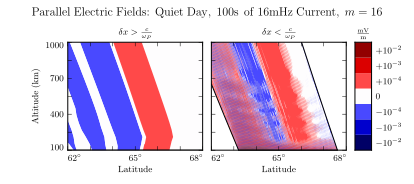
\includegraphics[width=\textwidth]{figures/inertial_length.pdf}
    \caption[Parallel Electric Fields by Perpendicular Grid Resolution]{
      The parallel electric field develops significant structure when the perpendicular grid resolution is smaller than the electron inertial length. Unfortunately, such runs are prohibitively expensive. The lower panel -- which still fails to resolve wave structure properly -- represents a 100-fold increase in computational time. 
    }
    \label{fig_inertial_length}
\end{figure}

Even so, the run presents a significant computational expense. Spread over 16 cores, a \SI{100}{\s} run on Tuna's usual grid takes well under an hour. The inertial-scale run barely finished in 96 hours, the cutoff at the Minnesota Supercomputing Institute\footnote{Runtime goes as the inverse square of grid resolution. Not only does finer resolution require more grid cells, but it also gives rise to proportionally smaller crossing times, imposing a smaller time step. }.

The snapshot shown in \cref{fig_inertial_length} uses a perpendicular grid resolution of \SI{0.7}{\km} at the Earthward edge, which just satisfies the Nyquist rate for the minimum inertial length of \SI{1.7}{\km}. It's still too coarse. There is clearly some small-scale structure developing in the ionosphere, but it's not well resolved. The large number of ``wigglies'' portends an imminent crash. 

Electron inertial effects present a promising first-principles-based approach to investigate parallel currents and electric fields associated with field line resonances. Unfortunately, because of the large differences in scale between Pc4 pulsations and the plasma oscillation, the proper deployment of inertial effects presents a prohibitive computational expense. For this reason, results presented in \cref{ch_results} make use of the core version of Tuna presented in \cref{sec_tuna}, which does not include the effects of electron inertia. 





% %%%%%%%%%%%%%%%%%%%%%%%%%%%%%%%%%%%%%%%%%%%%%%%%%%%%%%%%%%%%%%%%%%%%%%%%%%%%%
% %%%%%%%%%%%%%%%%%%%%%%%%%%%%%%%%%%%%%%%%%%%%%%%%%%%%%%% Building on Mann 1995
% %%%%%%%%%%%%%%%%%%%%%%%%%%%%%%%%%%%%%%%%%%%%%%%%%%%%%%%%%%%%%%%%%%%%%%%%%%%%%

\chapter{Results}
  \label{ch_azm}

\todo{This chapter is the real moneymaker. The overarching motivation for this work is that Pc4 pulsations vary in interesting ways with respect to azimuthal modenumber, and that prior models have been unable to give a good picture of that behavior. }

%\todo{Do we every check E/B against $\Sigma_P / \mz$? }

%\todo{Do we see a difference between \vec{k} (momentum) and the group velocity? Poynting flux will always be pretty much along the field line, since $B_3$ is small and $E_3$ is zero, but the wave vector need not be. This is a question of coupling/converting to compressional waves, I guess. }

%\todo{Look at McKenzie and Westphal. Waves incident on the bow shock, etc, at weird angles. }

%\todo{Look at the E to B ratio. Compare to the \Alfven speed and to the height-integrated Pedersen conductivity. }

% =============================================================================
% =============================================================================
% =============================================================================
%\section{Electromagnetic Energy Gap}

%\todo{A preliminary search (and asking Bob) has not turned up anyone looking at this before, so it's hard to provide context. }

%Above, we considered the decay of energy from the poloidal mode to the toroidal mode. A natural follow up is, are there any other surprising trends in the distribution of energy?

%As it turns out, yes!

%In cases where the driving frequency does not line up with the local bounce frequency, energy doesn't accumulate particularly well in either the poloidal or the toroidal mode. Like a damped-driven oscillator, the system's behavior follows the input. 

%At low \azm, what energy there is divides itself more or less equally between the electric and magnetic fields. 

%As \azm increases, oddly, a gap appears. When the conductivity is high, the magnetic field holds more energy than the electric field. The disparity can be up to a factor of $\sim \num{3}$; that is, \SI{75}{\percent}. of the energy in the magnetic field, and \SI{25}{\percent} in the electric field. When conductivity is low, the opposite happens: energy concentrates in the electric field. 

%This lines up somewhat with what might be expected. When conductivity is low, it takes a larger electric field to induce the same current, and thus the same magnetic field. But it's not clear why this disparity only appears at large \azm, or why it does not appear when the driving is resonant. 

%Maybe it's a timing issue? A relationship between the bounce time (which is more or less indepedent of \azm) and the rotation time (which depends on \azm). 

%\todo{How is the compressional magnetic field brought into these calculations? It exists only at small \azm. It's never particularly large, it also gets added to the zeroth-order field before squaring. }

%\begin{figure}[H]
%    \centering
%    \includegraphics[width=\textwidth]{figures/U_BE_010mHz.pdf}
%    \caption[Current-Driven Electric and Magnetic Energy: 10mHz]{
%      In the absence of resonant driving, a disparity emerges at large \azm between the energy in the magnetic field and the energy in the electric field. The sign of the difference depends on the ionospheric conductivity. 
%    }
%    \label{fig_U_BE_010mHz}
%\end{figure}

%\begin{figure}[H]
%    \centering
%    \includegraphics[width=\textwidth]{figures/U_BE_022mHz.pdf}
%    \caption[Current-Driven Electric and Magnetic Energy: 22mHz]{
%      When driving is resonant, energy is distributed almost exactly half-and-half between the electric and magnetic fields, regardless of \azm. The rightmost profile still shows a gap, likely because the ionospheric conductivity in that model is low enough that nothing ever resonates. 
%    }
%    \label{fig_U_BE_022mHz}
%\end{figure}













  
% =============================================================================
% =============================================================================
% =============================================================================
\section{Finite Poloidal Lifetimes}
  \label{sec_lifetimes}

Radoski\cite{radoski_1974} looked at \Alfven waves, using a cylindrical coordinate system to imitate an ``unwrapped'' dipole. He argued that poloidal waves should asymptotically rotate to the toroidal mode. 

Mann\cite{mann_1995} performed some wave-in-a-box simulations and found the rotation time to be linear in modenumber: $\tau = \frac{d \lambda}{d \omega_A'}$, where $\lambda = \frac{\azm}{2 \pi r}$ and $\omega_A'$ is the spatial derivative of the \Alfven bounce frequency. Soon afterwards\cite{mann_1997}, he supported his simulations analytically. 

\todo{Crunch out $\frac{d \lambda}{d \omega_A'}$. Preliminary indications are that it doesn't translate well to a realistic grid, but let's double check. }

Ding\cite{ding_1995} ran simulations more-or-less concurrent with Mann's. Ding saw a rotation from poloidal to toroidal... then back again. It seems that the reversal was a spatial resolution issue. 

The aforementioned models made significant simplifying assumptions in terms of geometry and boundary conditions. 

Mann used straight field lines, a uniform \Alfven speed gradient, and perfectly conducting boundaries. 

Ding's simulation is nominally carried out in a dipole geometry, but the ionospheric boundary is at \SI{2.5}{\RE}. Boundaries are also perfectly conducting. 

That is, the results below offer a significantly higher level of realism than any past simulation (in part, of course, because computers are a lot better than they were 20 years ago). 

A dedicated 3D treatment of this problem is unlikely at present. Large azimuthal modenumbers are expensive to compute. That's the whole point! 

The energy is obtained by integrating (using the Jacobian to handle the grid properly) $U = \int dU = \int u \, dV$. Values are the log (base 10) of that, in the slightly odd units of gigajoules per radian. A factor of $2\pi$ wouldn't change anything, of course, but it seems inappropriate to integrate all the way around the sphere when Pc4s are longitudinally localized (a fact which was an important part of justifying a 2.5D approach). 

% -----------------------------------------------------------------------------
% -----------------------------------------------------------------------------
% -----------------------------------------------------------------------------
\subsection{High Conductivity}

In \cref{fig_U_day}, the rotation of energy from the poloidal mode to the toroidal mode is clear. Driving is strictly poloidal, yet the toroidal mode accumulates energy over time, and doesn't appear to give it back. The rotation happens faster for low-\azm simulations, qualitatively consistent with Mann's result; the time at which poloidal and toroidal energies are equal seems to even be linear in \azm, in line with his result. 

At least, this is the case on the dayside, where the ionosphere is highly conductive. 

\begin{figure}[H]
    \centering
    \includegraphics[width=\textwidth]{figures/U_1.pdf}
    \caption[Poloidal and Toroidal Energy: Active Day]{
      Driving -- delivered to the poloidal mode -- asymptotically rotates to the toroidal mode. The rate of rotation is strongly affected by the azimuthal modenumber. 
    }
    \label{fig_U_day}
\end{figure}

\todo{Talk about why this is exciting. }

\todo{Note that Mann looked specifically at second-harmonic waves. }

\todo{This result shows agreement with -- and significant refinement of -- Mann's findings. In the case of large-but-finite ionospheric conductivity, dipole geometry, and realistic \Alfven speed profile, energy does asymptotically rotate from the poloidal mode to the toroidal mode. The rotation rate is strongly affected by azimuthal modenumber and, in the case of large-but-finite \azm, has a characteristic timescale in the tens of periods. The present work furthermore demonstrates that the rotation rate is affected by driving frequency (did Mann talk about this at all, or just work in normalized time?) }

% -----------------------------------------------------------------------------
% -----------------------------------------------------------------------------
% -----------------------------------------------------------------------------
\subsection{Low Conductivity}

The picture on the nightside (where the ionospheric conductivity is low) is significantly different from the dayside (where it's high). 

Dissipation seems to outstrip rotation. Energy does not accumulate over numerous driving periods, as would be expected in resonance; it follows the driving up and down, as a damped-driven oscillator. 

There is evidence that the rotation is still trying to happen. At low \azm, energy is distributed between the poloidal and toroidal mode before dissipating; at high \azm, the energy dissipates straight out of the poloidal mode, never having had a chance to rotate. 

\begin{figure}[H]
    \centering
    \includegraphics[width=\textwidth]{figures/U_4.pdf}
    \caption[Poloidal and Toroidal Energy: Quiet Night]{
      Driving is applied to the poloidal electric field. There is some rotation of energy to the toroidal mode (and less at high azimuthal modenumber), but the low ionospheric conductivity prevents energy from accumulating over time. 
    }
    \label{fig_U_night}
\end{figure}

\todo{Why is this exciting? }

\todo{Previous considerations of poloidal lifetimes have been limited to the high conductivity regime. The present work demonstrates that the low conductivity regime exhibits qualitative differences. Ionospheric conductivity on the nightside is low enough that resonance does not develop, even in the case of ongoing driving. The dissipation timescale is comparable to the rotation timescale. Rather than aymoptotically accumulating energy in the toroidal mode, the oscillator asymptotically oscillates following the driving. This is relevant to the question of day-night asymmetry in the observation of field line resonances. }


  
% =============================================================================
% =============================================================================
% =============================================================================
\section{Spatial Distribution of Energy}
  \label{sec_shells}

Looking a bit deeper, it's possible to comment on the structure of the poloidal and toroidal modes, not just their magnitudes. The following commentary addresses the dayside; on the nightside, there's never much by the way of resonance. 

In \cref{fig_resonant_driving,fig_nonresonant_driving}, electromagnetic energy is binned by field line, averaged over volume (again, with respect to the Jacobian), and plotted as contours. All plots share a color scale. 

The poloidal mode and the toroidal mode exhibit qualitatively different behavior, related to the fact that energy rotates from poloidal to toroidal, and not back. 

At low \azm, energy rotates out of the poloidal mode so quickly that no resonance can form. 

At high \azm, the \Alfven wave is guided. If the driving frequency lines up with the resonant frequency where it's delivered, the poloidal mode resonates strongly. Otherwise, again, no energy accumulates. 

In no case does the poloidal mode demonstrate the ability to move energy across magnetic field lines. 

On the other hand, the toroidal mode does resonate, even if the driving isn't resonant (though in that case the response is of course stronger). The toroidal mode transports energy across field lines until it encounters resonance, then accumulates energy there. Often, resonances are seen in multiple locations due to the non-monotonic \Alfven bounce frequency (recall \cref{fig_fa}) as a function of $L$. 

% -----------------------------------------------------------------------------
% -----------------------------------------------------------------------------
% -----------------------------------------------------------------------------
\subsection{Resonant Driving}

\begin{figure}[H]
    \centering
    \includegraphics[width=\textwidth]{figures/layers_22mHz_1.pdf}
    \caption[Poloidal and Toroidal Energy Distribution: Resonant Driving]{
      If \azm is small, energy rotates to the toroidal mode too fast to form a poloidal resonance. If \azm is large, the \Alfven wave is guided, so it resonates only if the driving frequency lines up with the resonant frequency where it's applied. The result is just one big -- or perhaps even giant -- pulsation. If the driving lines up with a nearby field line, the toroidal mode goes crazy! Resonance inside the plasmasphere. Resonance at the plasmapause. Resonance at the driving location. And (weak) attempt at a higher harmonic further out. 
    }
    \label{fig_resonant_driving}
\end{figure}

\todo{Why is this exciting? }

\todo{Driving from inside the magnetosphere is novel. }

% -----------------------------------------------------------------------------
% -----------------------------------------------------------------------------
% -----------------------------------------------------------------------------
\subsection{Nonresonant Driving}

\begin{figure}[H]
    \centering
    \includegraphics[width=\textwidth]{figures/layers_13mHz_2.pdf}
    \caption[Poloidal and Toroidal Energy Distribution: Nonresonant Driving]{
      When the driving frequency doesn't line up with the location where it's delivered, there's basically no response. There is no movement of energy to a resonant field line, so no energy can accumulate over the course of multiple rounds of driving. Even when not driven resonantly, the toroidal mode still makes the best of its situation. It steals what energy it can from the poloidal mode, carries it to the resonant $L$-shell, and gets to work. (In contrast, recall from \cref{fig_resonant_driving}, in this situation the poloidal mode just does not accumulate energy.)
    }
    \label{fig_nonresonant_driving}
\end{figure}

\todo{Why is this exciting? }


  
% =============================================================================
% =============================================================================
% =============================================================================
\section{Significance for Giant Pulsations}
  \label{sec_pgs}

Giant pulsations are (probably\cite{takahashi_2011}) fundamental mode poloidal Pc4 pulsations with frequencies around \SI{10}{\mHz} and azimuthal modenumbers around \num{20}. They are large, and can sometimes be observed on the ground. 

While this model makes no particular distinction between a giant pulsation and any other Pc4, the above results do line up with giant pulsation observations. 

Giant pulsations aren't seen at small \azm. As shown in \cref{sec_lifetimes}, low-\azm poloidal modes rotate to the toroidal mode too quickly to resonate effectively, even in the case of continuous driving at a locally-resonant frequency. The sweet spot seems to be around $\azm = 20$, more or less the same point where resonance becomes visible in \cref{fig_resonant_driving}. Admittedly, giant pulsations are typically closer to \SI{10}{\mHz} than \SI{22}{\mHz}. It seems likely that qualitatively similar results would be encountered if the driving were moved to an $L$-shell with a bounce time of \SI{10}{\mHz}. 

% -----------------------------------------------------------------------------
% -----------------------------------------------------------------------------
% -----------------------------------------------------------------------------
\subsection{Ground Signatures}

\todo{\cite{takahashi_2011} talks significantly about the east-west polarization. }

Giant pulsations are seen at very large \azm, though not on the ground\cite{takahashi_2013}, due to damping by the ionosphere. 

Giant pulsations are most common on the dayside (particularly the morningside), during geomagnetically quiet times. Giant pulsation ground signatures are noted for their predisposition towards east-west polarization. 

In \cref{fig_ground_signatures}, the strongest east-west ground signatures is obtained on the geomagnetically quiet dayside, at \azm of 16 and 32. 

This seems to be a giant pulsation ``sweet spot'': the poloidal mode becomes stronger as \azm increases, but the ionospheric damping also increases. 

\begin{figure}[H]
    \centering
    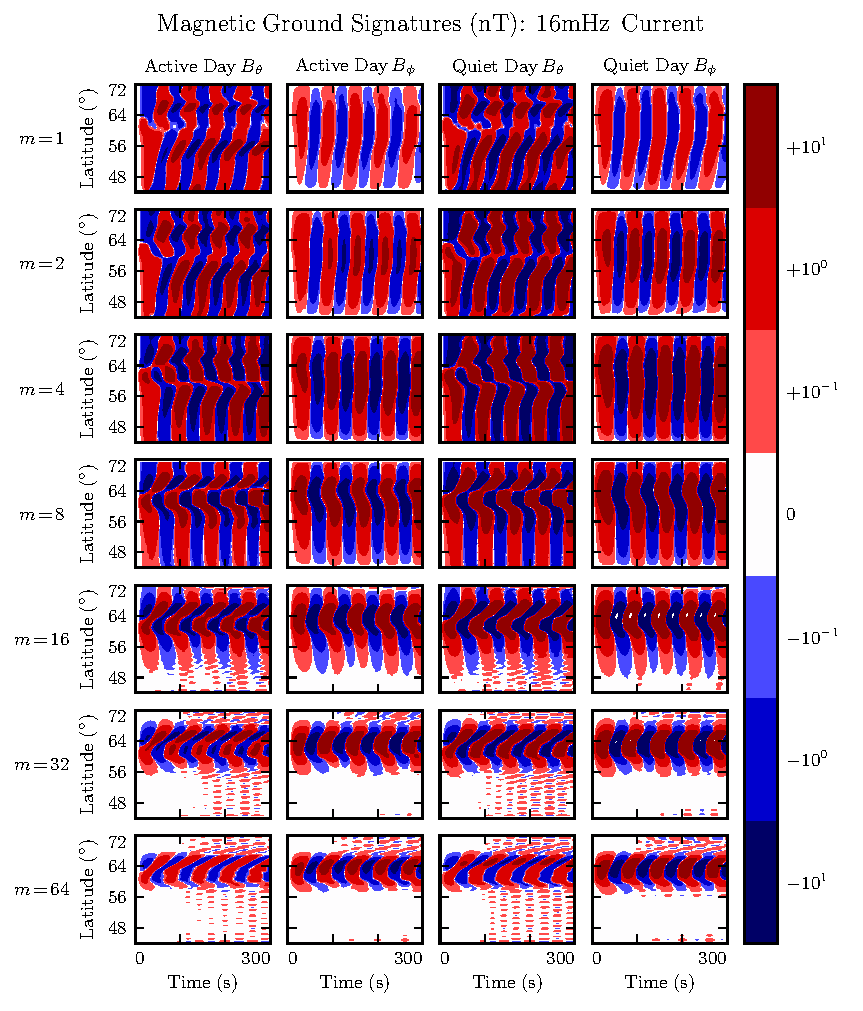
\includegraphics[width=\textwidth]{figures/ground_16mHz.pdf}
    \caption[Dayside Ground Magnetic Fields]{
      The east-west component of magnetic ground signatures is peaked on the geomagnetically quiet dayside, at modenumbers around 16 to 32. This coincides nicely with observations of giant pulsations. Like the east-west component, the north-south ground signature is strongest on the quiet dayside; however, unlike the east-west component, the north-south component is weak when the modenumber is large. 
    }
    \label{fig_ground_signatures}
\end{figure}

Giant pulsations are monochromatic, and can be accompanied by ``multiharmonic toroidal waves''\cite{takahashi_2011}. Per \cref{sec_shells}, this is about what would be expected from a mishmash of poloidal driving. Poloidal modes of all frequencies rotate into the toroidal mode; resonant poloidal modes resonate; non-resonant poloidal modes become evanescent. 

Giant pulsations often drift azimuthally. This model can't resolve azimuthal drift directly, of course, but can fake it by looking at complex phase. There has been some indication (not shown) of complex phase rotation in ground magnetic fields. However, at the boundary, it's difficult to disentangle which values are imaginary to indicate an azimuthal offset, and which are imaginary because of Hall coupling. Investigation is ongoing. 




% %%%%%%%%%%%%%%%%%%%%%%%%%%%%%%%%%%%%%%%%%%%%%%%%%%%%%%%%%%%%%%%%%%%%%%%%%%%%%
% %%%%%%%%%%%%%%%%%%%%%%%%%%%%%%%%%%%%%%%%%%%%% Validate the Model Against RBSP
% %%%%%%%%%%%%%%%%%%%%%%%%%%%%%%%%%%%%%%%%%%%%%%%%%%%%%%%%%%%%%%%%%%%%%%%%%%%%%

\chapter{Observations}
  \label{ch_rbsp}

\todo{Talk about recent surveys by Dai\cite{dai_2015} and Motoba\cite{motoba_2015}. Note that they skirt the issue of the fundamental mode in general. Everyone talks about how Pgs are rare... but how rare are they compared to the fundamenal poloidal Pc4 in general? }








% %%%%%%%%%%%%%%%%%%%%%%%%%%%%%%%%%%%%%%%%%%%%%%%%%%%%%%%%%%%%%%%%%%%%%%%%%%%%%
% %%%%%%%%%%%%%%%%%%%%%%%%%%%%%%%%%%%%%%%%%%%%%%%%%%%%%%%%%%%%%%%%%% Conclusion
% %%%%%%%%%%%%%%%%%%%%%%%%%%%%%%%%%%%%%%%%%%%%%%%%%%%%%%%%%%%%%%%%%%%%%%%%%%%%%

\chapter{Conclusion}
  \label{ch_conclusion}




% Bibliography
\bibliography{thesis}

% Appendices
\appendix

% %%%%%%%%%%%%%%%%%%%%%%%%%%%%%%%%%%%%%%%%%%%%%%%%%%%%%%%%%%%%%%%%%%%%%%%%%%%%%
% %%%%%%%%%%%%%%%%%%%%%%%%%%%%%%%%%%%%%%%%%%%%% Appendix: Differential Geometry
% %%%%%%%%%%%%%%%%%%%%%%%%%%%%%%%%%%%%%%%%%%%%%%%%%%%%%%%%%%%%%%%%%%%%%%%%%%%%%

\chapter{Differential Geometry}
\label{app_geometry}

\todo{Not sure that a glossary or list of acronyms will be necessary, but here are the examples from the template. }

\section{Glossary}
\label{jargonapp}
\begin{itemize}
\item \textbf{Cosmic-Ray Muon} (\textbf{CR $\mu$}) -- A muon coming from
the abundant energetic particles originating outside of the Earth's
atmosphere.
\end{itemize}

\section{Acronyms}
\label{acronymsec}

% Heading for the first page
\begin{longtable}{p{0.25\textwidth} p{0.75\textwidth}}
\caption{Acronyms} \label{tab:acronyms} \\

\toprule
Acronym & Meaning \\
\midrule
\endfirsthead

% Heading for all subsequent pages
\multicolumn{2}{l}{\textit{\tablename\ \thetable{} -- Continued from previous page}} \\
\toprule
Acronym & Meaning \\
\midrule
\endhead

% Footer for each page that wraps over to the next
\multicolumn{2}{r}{\textit{Continued on next page}} \\
\bottomrule
\endfoot

% Footer for the end of the table
\bottomrule
\endlastfoot

% End table formatting

CR$\mu$ & Cosmic-Ray Muon \\

\end{longtable}



%% %%%%%%%%%%%%%%%%%%%%%%%%%%%%%%%%%%%%%%%%%%%%%%%%%%%%%%%%%%%%%%%%%%%%%%%%%%%%%
% %%%%%%%%%%%%%%%%%%%%%%%%%%%%%%%%%%%%%%%%%%%%%%% Appendix: Integrating Factors
% %%%%%%%%%%%%%%%%%%%%%%%%%%%%%%%%%%%%%%%%%%%%%%%%%%%%%%%%%%%%%%%%%%%%%%%%%%%%%








\chapter{Integrating Factors}
\label{app_integrating}

Start with differential equation of the form:

\begin{align}
  \frac{\partial}{\partial t} X(t) + \alpha X(t) &= \beta
\end{align}

Multiply by the integrating factor, then group terms: 

\begin{align}
  \exp (\alpha \; t) \frac{\partial}{\partial t} X(t) + \alpha \exp(\alpha \; t) X(t) &= \beta \exp(\alpha \; t) \\
  \frac{\partial}{\partial t} \big[ \exp(\alpha t) X(t) \big] &= \beta \exp(\alpha t)
\end{align}

Integrate from 0 to $\delta t$, assuming that $\beta$ is constant in time or varies slowly. 

\begin{align}
  \int^{\delta t}_0 dt \frac{\partial}{\partial t} \big[ \exp(\alpha t) X(t) \big] &= \int^{\delta t}_0 dt \beta \exp(\alpha t) \\
  \exp (\alpha \deltat) X(\deltat) - X(0) &= \deltat \beta ( \frac{\deltat}{2} ) \exp ( \alpha \frac{\deltat}{2} )
\end{align}

Then rearrange to solve for the new value of X:

\begin{align}
  X(\delta t) &= X(0) \exp ( -\alpha \delta t ) + \delta t \beta ( \frac{\delta t}{2} ) \exp ( -\alpha \frac{\delta t}{2} )
\end{align}

Done. 


% End the Document
\end{document}




